\documentclass{article}
%% Chapter 1 Section 10: Exponentiation

\usepackage{amsmath}
\usepackage{palatino}
\usepackage{tikz}

\newcommand{\curry}[1]{\emph{curry}(#1)}
\newcommand{\eval}{\emph{eval}}
\newcommand{\id}{\emph{id}}
\newcommand{\cset}{\mathbf{Set}}
\newcommand{\csetset}{\cset \times \cset}
\begin{document}

\begin{enumerate}
\item [1.10.5.1]
\item [1.10.5.2]
  Exponentation in $\csetset$ is componentwise.
  That is, every pair of $\csetset$ objects determines an exponential.
  
  Let $A \times B$ and $C \times D$ be two objects in $\csetset$.
  The exponential of this pair is an object $C^A \times D^B$.
  The function $\eval$  has domain $(C^A \times D^B) \times (A \times B)$ and codomain $C \times D$.
  Application is componentwise.
  The result of $\eval((f, g), (a,b))$ is the pair $(f a, g b)$.

  Then for every arrow $g : E \times (A \times B) \rightarrow C \times D$, we have a unique arrow $\curry{g}$ that maps the $\csetset$ object $E$ to the exponential $C^A \times D^B$.
  This arrow is uniquely determined comoponentwise; because $E$ is itself a pair of $\cset$ objects, each with an exponential, we obtain the $csetset$ object by taking the exponential of the first and second member of the pair.
  
  The entire construction is summarized in the below diagram.
  Parenthesis are inserted for readability.
  \begin{center}
    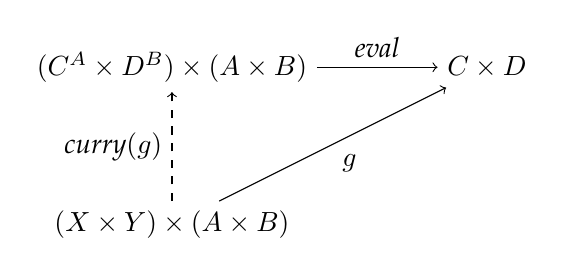
\begin{tikzpicture}
      \node (1) {$(C^A \times D^B) \times (A \times B)$};
      \node[below of=1, yshift=-1cm] (2) {$(X \times Y) \times (A \times B)$};
      \node[right of=1,xshift=3cm] (3) {$C \times D$};
      
      \draw[->] (1) -- node[above] {$\eval$} (3);
      \draw[->] (2) -- node[below right] {$g$} (3);
      \draw[->,dashed] (2) -- node[left] {$\curry{g}$} (1);
    \end{tikzpicture}
  \end{center}

\item [1.10.5.3]
\item [1.10.5.4]
  To show that $\curry{\eval_{AB}} = \id_{(B^A)}$, we fill blanks in the exponent diagram.
  \begin{center}
    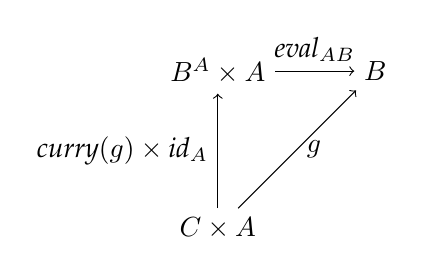
\begin{tikzpicture}
      \node (1) {$B^A \times A$};
      \node [below of=1,yshift=-1cm] (2) {$C \times A$};
      \node [right of=1,xshift=1cm] (3) {$B$};
      
      \draw[->] (2) -- node [right] {$g$} (3);
      \draw[->] (2) -- node [left] {$\curry{g} \times \id_A$} (1);
      \draw[->] (1) -- node [above] {$\eval_{AB}$} (3);
    \end{tikzpicture}
  \end{center}

  In this case, we want to curry the eval function.
  Hence we replace $g$ with $\eval_{AB}$.
  This constricts the domain of $\curry{\eval_{AB}}$ to be $(B^A \times A)$, same as its codomain.
  As $\curry{}$ is unique and shares its domain and codomain with $\id_{B^A}$, it must be the case that $\curry{\eval_{AB}} = id_{B^A}$.
  \begin{center}
    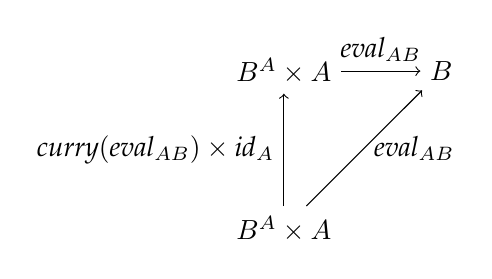
\begin{tikzpicture}
      \node (1) {$B^A \times A$};
      \node [below of=1,yshift=-1cm] (2) {$B^A \times A$};
      \node [right of=1,xshift=1cm] (3) {$B$};
      
      \draw[->] (2) -- node [right] {$\eval_{AB}$} (3);
      \draw[->] (2) -- node [left] {$\curry{\eval_{AB}} \times \id_A$} (1);
      \draw[->] (1) -- node [above] {$\eval_{AB}$} (3);
    \end{tikzpicture}
  \end{center}

\item [1.10.5.5]
\item [1.10.5.6]
\item [1.10.5.7]
\item [1.10.5.8]
\end{enumerate}

\end{document}
